\documentclass{standalone}

\usepackage{tikz}
\usetikzlibrary{matrix}
\usetikzlibrary{positioning}
\usetikzlibrary{shapes}
\usepackage{times} % To change font to times
\usetikzlibrary{trees,positioning,shapes,shadows,arrows}
\usepackage{circuitikz}

\begin{document}

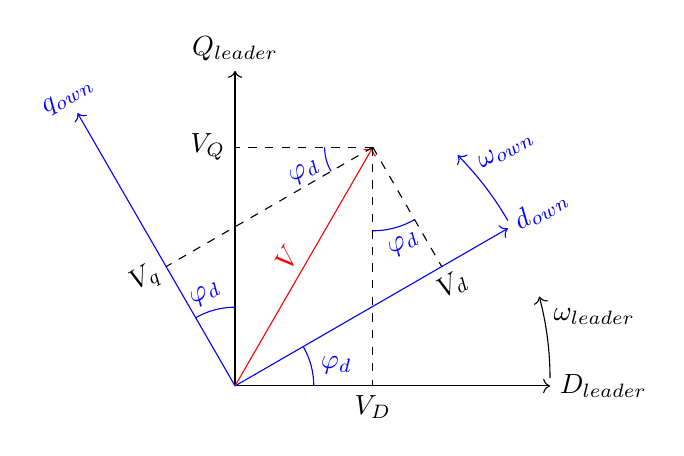
\begin{tikzpicture}
    % Parameters -- Unexpected behaviour if angles are > 90 or < 0
    \pgfmathsetmacro{\angleown}{30}
    \pgfmathsetmacro{\lengthaxis}{4}
    \pgfmathsetmacro{\angleV}{60} % should be higher than \angleown
    \pgfmathsetmacro{\lengthV}{3.5}
    
    
    % Let's draw!
\draw[->] (0,0) -- (\lengthaxis,0)  node[right] {$D_{leader}$};
   	    \draw[->] (0,0) -- (0,\lengthaxis)  node[above] {$Q_{leader}$};
   	    \draw[->,blue] (0,0) -- ({\lengthaxis*cos(\angleown)},{\lengthaxis*sin(\angleown)})  node[right,rotate=\angleown] {$d_{own}$};
   	    \draw[->,blue] (0,0) -- ({-\lengthaxis*sin(\angleown)},{\lengthaxis*cos(\angleown)})  node[above,rotate=\angleown] {$q_{own}$};
   	    \draw[-,blue] (0.25*\lengthaxis,0) arc (0:\angleown:0.25*\lengthaxis) node[midway,right] {$\varphi_{d}$};
   	    \draw[-,blue] (0,0.25*\lengthaxis) arc (90:90+\angleown:0.25*\lengthaxis) node[midway,above,rotate=\angleown] {$\varphi_{d}$};
   	    \draw[-,blue] ({\lengthV*cos(\angleV)},{0.65*\lengthV*sin(\angleV)}) arc (270:270+\angleown:{0.35*\lengthV*sin(\angleV)}) node[midway,below,rotate=\angleown] {$\varphi_{d}$};
   	    \draw[-,blue] ({0.65*\lengthV*cos(\angleV)},{\lengthV*sin(\angleV)}) arc (180:180+\angleown:{0.35*\lengthV*cos(\angleV)}) node[midway,left,rotate=\angleown] {$\varphi_{d}$};
   	    \draw[->,red] (0,0) -- ({\lengthV*cos(\angleV)},{\lengthV*sin(\angleV)})  node[midway,above,rotate=\angleV] {$V$};
   	    \draw[->,black] (\lengthaxis,0.1) arc (0:15:\lengthaxis) node[near end,right] {$\omega_{leader}$};
   	    \draw[->,blue] ({\lengthaxis*cos(\angleown)},{\lengthaxis*sin(\angleown)+0.1}) arc (\angleown:\angleown+15:\lengthaxis) node[near end,right,rotate=\angleown] {$\omega_{own}$};   
   	    
   	    % Dashed lines (coordinates)
   	    \draw[dashed] ({\lengthV*cos(\angleV)},{\lengthV*sin(\angleV)}) -- ({\lengthV*cos(\angleV)},0)  node[below] {$V_D$};	
   	    \draw[dashed] ({\lengthV*cos(\angleV)},{\lengthV*sin(\angleV)}) --       (0,{\lengthV*sin(\angleV)})  node[left] {$V_Q$};
   	    \draw[dashed] ({\lengthV*cos(\angleV)},{\lengthV*sin(\angleV)}) -- ({\lengthV*cos(\angleV-\angleown)*cos(\angleown)},{\lengthV*cos(\angleV-\angleown)*sin(\angleown)})  node[below,rotate=\angleown] {$V_d$};	
   	    \draw[dashed] ({\lengthV*cos(\angleV)},{\lengthV*sin(\angleV)}) --       ({-\lengthV*sin(\angleV-\angleown)*sin(\angleown)},{\lengthV*sin(\angleV-\angleown)*cos(\angleown)})  node[left,rotate=\angleown] {$V_q$};    
\end{tikzpicture}


\end{document}